\newsection{Amazon Web Services}
Amazon Web Services (AWS) is a subsidiary of Amazon that provides on-demand cloud computing platforms to individuals, companies, and governments, on a pay-as-you-go basis. These cloud computing web services provide a set of primitive abstract technical infrastructure and distributed computing building blocks and tools. AWS's version of virtual computers emulate most of the attributes of a real computer including, hardware central processing units and graphics processing units, local/RAM memory, hard-disk/SSD storage; a choice of operating systems; networking; and pre-loaded application software such as web servers and databases.

\subsection{Lambda}
AWS Lambda is an event-driven, serverless computing platform provided by Amazon. It is a computing service that runs code in response to events and automatically manages the computing resources required by that code. The purpose of Lambda is to simplify building smaller, on-demand applications that are responsive to events and new information. AWS targets starting a Lambda instance within milliseconds of an event. Node.js, Python, Java, Go, Ruby and C\# through .NET Core are all officially supported.\\

In this project, lambda functions are the computing core for the execution of all commands and are written in Node.js.

\subsubsection{Write mode Lambda functions}
\paragraph{PushOperationAggregateToSQS} \Spazio
This functions starts the flow and triggered when fetching the corresponding API gateway URL with a POST request like this: \\
\begin{figure} [H]
	\centering
	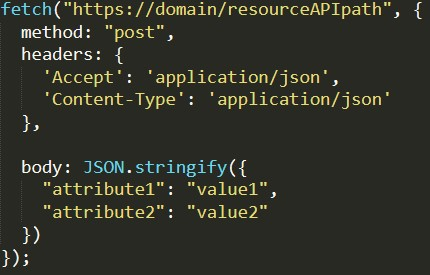
\includegraphics[scale=1.2]{../Img/fetchPOST}
	\caption{Fetch POST API}\label{}
\end{figure}
Once triggered, this functions retrieve the event and put it in the \emph{MessageBody} parameter. The event object is not changed, instead in the user functions which encrypt the password before sending the message to corresponding SQS queue.


\paragraph{CommandOperationAggregate} \Spazio
This functions validate the values of the attributes before storing the event in the \emph{eventStore} and triggered when a new event arrives to the corresponding queue. \\ 
If you have to check for duplicated attributes in the database, the function must be marked \emph{async} because it has to wait for the result of the check operation.

\paragraph{Mediator} \Spazio
This function catch the \emph{DynamoDB} event and triggered when a change occurs in a certain table. \\
You have to be careful that the \emph{DynamoDB} events are mapped using the char type attribute value. This is an example:

After that, the \emph{QueueUrl} parameter retrieved from the event objec, the payload event is passed with the \emph{MessageBody} and then sending the execution message to corresponding SQS queue. 

\paragraph{OperationAggregate}


\paragraph{recovery}

\subsubsection{Read mode Lambda functions}
\paragraph{readOperation}


\subsubsection{CloudWatch Logs}


\subsection{DynamoDB}

\subsection{API Gateway}

\subsection{Simple Queue Service}
